\documentclass[10pt,handout]{beamer}\usepackage[]{graphicx}\usepackage[]{color}
% maxwidth is the original width if it is less than linewidth
% otherwise use linewidth (to make sure the graphics do not exceed the margin)
\makeatletter
\def\maxwidth{ %
  \ifdim\Gin@nat@width>\linewidth
    \linewidth
  \else
    \Gin@nat@width
  \fi
}
\makeatother

\definecolor{fgcolor}{rgb}{0.345, 0.345, 0.345}
\newcommand{\hlnum}[1]{\textcolor[rgb]{0.686,0.059,0.569}{#1}}%
\newcommand{\hlstr}[1]{\textcolor[rgb]{0.192,0.494,0.8}{#1}}%
\newcommand{\hlcom}[1]{\textcolor[rgb]{0.678,0.584,0.686}{\textit{#1}}}%
\newcommand{\hlopt}[1]{\textcolor[rgb]{0,0,0}{#1}}%
\newcommand{\hlstd}[1]{\textcolor[rgb]{0.345,0.345,0.345}{#1}}%
\newcommand{\hlkwa}[1]{\textcolor[rgb]{0.161,0.373,0.58}{\textbf{#1}}}%
\newcommand{\hlkwb}[1]{\textcolor[rgb]{0.69,0.353,0.396}{#1}}%
\newcommand{\hlkwc}[1]{\textcolor[rgb]{0.333,0.667,0.333}{#1}}%
\newcommand{\hlkwd}[1]{\textcolor[rgb]{0.737,0.353,0.396}{\textbf{#1}}}%
\let\hlipl\hlkwb

\usepackage{framed}
\makeatletter
\newenvironment{kframe}{%
 \def\at@end@of@kframe{}%
 \ifinner\ifhmode%
  \def\at@end@of@kframe{\end{minipage}}%
  \begin{minipage}{\columnwidth}%
 \fi\fi%
 \def\FrameCommand##1{\hskip\@totalleftmargin \hskip-\fboxsep
 \colorbox{shadecolor}{##1}\hskip-\fboxsep
     % There is no \\@totalrightmargin, so:
     \hskip-\linewidth \hskip-\@totalleftmargin \hskip\columnwidth}%
 \MakeFramed {\advance\hsize-\width
   \@totalleftmargin\z@ \linewidth\hsize
   \@setminipage}}%
 {\par\unskip\endMakeFramed%
 \at@end@of@kframe}
\makeatother

\definecolor{shadecolor}{rgb}{.97, .97, .97}
\definecolor{messagecolor}{rgb}{0, 0, 0}
\definecolor{warningcolor}{rgb}{1, 0, 1}
\definecolor{errorcolor}{rgb}{1, 0, 0}
\newenvironment{knitrout}{}{} % an empty environment to be redefined in TeX

\usepackage{alltt}


%\input{slides_header.tex}
\usepackage{graphicx}
\usepackage{hyperref, url}
\hypersetup{colorlinks,citecolor=myorange,filecolor=red,linkcolor=brown,urlcolor=blue}

\usepackage{longtable,booktabs}
\usepackage{amssymb,amsmath}
\usepackage{animate}
\usepackage{subfig}
\usepackage{tikz}
\usetikzlibrary{shapes.geometric, arrows,shapes.symbols,decorations.pathreplacing}
\tikzstyle{startstop} = [rectangle, rounded corners, minimum width=3cm, minimum height=1cm, draw=black, fill=pinkish,text width=3.5cm]
\tikzstyle{startstop2} = [rectangle, rounded corners, minimum width=3cm, minimum height=1cm, draw=black, fill=background,text width=4.5cm]
\tikzstyle{startstop3} = [rectangle, rounded corners, minimum width=3cm, minimum height=1cm, draw=black, fill=beige,text width=3.0cm]
\tikzstyle{startstop4} = [rectangle, rounded corners, minimum width=3cm, minimum height=1cm, draw=black, fill=pinkish,text width=4.5cm]
\tikzstyle{io} = [trapezium, trapezium left angle=70, trapezium right angle=110, minimum width=2cm, minimum height=1cm, text centered, draw=black, fill=blue!30,text width=1.5cm]
\tikzstyle{process} = [rectangle, minimum width=1cm, minimum height=1cm, text centered, draw=black, fill=orange!30,text width=2cm]
\tikzstyle{decision} = [diamond, minimum width=2cm, minimum height=1cm, text centered, draw=black, fill=green!30]
\tikzstyle{arrow} = [thick,->,>=stealth]
\tikzstyle{both} = [thick,<->,>=stealth, red]


% used for tree of stats tests in 001-introduction
\tikzstyle{startstopstats} = [rectangle, rounded corners, minimum width=2cm, minimum height=.5cm,text centered, draw=black, fill=red!30]
\tikzstyle{iostats} = [trapezium, trapezium left angle=70, trapezium right angle=110, minimum width=2cm, minimum height=.5cm, text centered, draw=black, fill=blue!30]
\tikzstyle{processstats} = [rectangle, minimum width=1.5cm, minimum height=.5cm, text centered, draw=black, fill=orange!30]
\tikzstyle{processbigstats} = [rectangle, minimum width=1.5cm, minimum height=.5cm, text centered, draw=black, fill=orange!30,text width=1.6cm]
\tikzstyle{decisionstats} = [rectangle, minimum width=1cm, minimum height=1cm, text centered, draw=black, fill=green!30,text width=1.6cm]
\tikzstyle{decisionbigstats} = [rectangle, minimum width=1cm, minimum height=1cm, text centered, draw=black, fill=yellow!30,text width=2cm]

\usepackage{pifont}% http://ctan.org/pkg/pifont
\newcommand{\cmark}{\ding{51}}%
\newcommand{\xmark}{\ding{55}}%

\usepackage{ulem} % for strikeout

\usepackage{xcolor}
\usepackage{color, colortbl}
\definecolor{lightgray}{RGB}{200,200,200}
\definecolor{palegray}{RGB}{221,221,221}
\definecolor{myblue}{RGB}{0,89,179}
\definecolor{myorange}{rgb}{0.776,0.357,0.157}
\definecolor{gray}{RGB}{110,110,110}
\definecolor{darkgray}{RGB}{100,100,100}
\definecolor{lightgray}{RGB}{200,200,200}
\definecolor{palegray}{RGB}{221,221,221}
\definecolor{turquoise}{RGB}{81,193,188}
\definecolor{tomato}{RGB}{255,136,136}
\definecolor{mandarina}{RGB}{229,169,25}
\definecolor{foreground}{RGB}{81,141,193}
\definecolor{background}{RGB}{246,244,240}
\definecolor{highlight}{RGB}{229,169,25}
\definecolor{lowlight}{RGB}{200,200,200}
\definecolor{beige}{RGB}{255,255,240}
\definecolor{pinkish}{RGB}{255,223,247}
\definecolor{darktangerine}{rgb}{1.0, 0.66, 0.07}
\definecolor{deepink}{RGB}{255,20,147}
%\usepackage{shadethm}
%\colorlet{shadecolor}{blue!15}
%\colorlet{shadecolor}{palegray}
%\setlength{\shadeboxrule}{.4pt}

%\newshadetheorem{thm}{Theorem}
%\newshadetheorem{defm}{Definition}
%\newshadetheorem{exm}{Exercise}
%\newshadetheorem{remarkm}{Remark}
%\definecolor{shadethmcolor}{HTML}{EDF8FF}
%\definecolor{shadethmcolor}{RGB}{221,221,221}
%\definecolor{shaderulecolor}{HTML}{45CFFF}
%\definecolor{shaderulecolor}{RGB}{0,89,179}
%\setlength{\shadeboxrule}{.4pt}



\usepackage{epsfig}

\newcommand{\code}[1]{\texttt{#1}}
\newcommand{\blue}[1]{\textcolor{blue}{#1}}
\newcommand{\red}[1]{\textcolor{red}{#1}}

\usepackage{comment}

\makeatletter

\def \iqsssectiontitleheader {}

\newcommand{\iqsssectiontitle}[1]{
	\def \iqsssectiontitleheader{#1}
}

\@ifundefined{insertmainframenumber}
{%
	% \insertmainframenumber not defined
	\newcommand{\insertmainframenumber}{\inserttotalframenumber}
}
{%
	% \insertmainframenumber already defined
}%


\AtBeginSection[]{
	\title{\insertsectionhead}
	{
		%\definecolor{white}{RGB}{140,193,250}
		%\definecolor{white}{RGB}{200,200,200}
		%\definecolor{white}{RGB}{242,244,247}
		\definecolor{white}{RGB}{0,89,179}
		%\definecolor{iqss@orange}{rgb}{1,1,1}
		\ifnum \insertmainframenumber > \insertframenumber
		%\setbeamercolor{background canvas}{bg=myblue}
		%\setbeamercolor{normal text}{fg=black,bg=white}
		%\setbeamercolor{frametitle}{fg=red}
		%\setbeamercolor{section in toc}{fg=myblue, bg=white}
		%\setbeamercolor{subsection in toc}{fg=myblue, bg=white}
		\frame{
			\frametitle{\iqsssectiontitleheader}
			\tableofcontents[currentsection]
		}
		\else
		\frame{
			\frametitle{Backup Slides}
			\tableofcontents[sectionstyle=shaded/shaded,subsectionstyle=shaded/shaded/shaded]
		}
		\fi
	}
}
\makeatother
%\graphicspath{{/home/sahir/git_repositories/EPIB607/resources/assets/slides/figure/}}


\usepackage{fontspec}
%\setsansfont{Fira Sans}
%\setmonofont{Fira Mono}
%\setsansfont[ItalicFont={Fira Sans Light Italic},BoldFont={Fira Sans},BoldItalicFont={Fira Sans Italic}]{Fira Sans Light}
%\setmonofont[BoldFont={Fira Mono Medium}]{Fira Mono}

\def\installpath{/usr/local/share/texmf/fonts/opentype/libertinus/}
\setmainfont{LibertinusSerif}[
UprightFont    = *-Regular,
BoldFont       = *-Bold,
ItalicFont     = *-Italic,
BoldItalicFont = *-BoldItalic,
Ligatures      = TeX,
Extension      = .otf,
Path           = \installpath/
]

\setsansfont{LibertinusSerif}[
UprightFont    = *-Regular,
BoldFont       = *-Bold,
ItalicFont     = *-Italic,
BoldItalicFont = *-BoldItalic,
Ligatures      = TeX,
Extension      = .otf,
Path           = \installpath/
]


%\setmonofont{LibertinusSerif}[
%UprightFont    = *-Regular,
%BoldFont       = *-Bold,
%ItalicFont     = *-Italic,
%BoldItalicFont = *-BoldItalic,
%Ligatures      = TeX,
%Extension      = .otf,
%Path           = \installpath/
%]






\newcommand\Wider[2][3em]{%
	\makebox[\linewidth][c]{%
		\begin{minipage}{\dimexpr\textwidth+#1\relax}
			\raggedright#2
		\end{minipage}%
	}%
}


\newcommand {\framedgraphic}[1] {
	\begin{figure}
		\centering
		\includegraphics[width=\textwidth,height=0.9\textheight,keepaspectratio]{#1}
	\end{figure}
}


\newcommand {\framedgraphiccaption}[2] {
	\begin{figure}
		\centering
		\includegraphics[width=\textwidth,height=0.8\textheight,keepaspectratio]{#1}
		\caption{#2}
	\end{figure}
}




\setbeamercolor{itemize item}{fg=myblue}
\setbeamercolor{itemize subitem}{fg=myorange}
%\setbeamertemplate{itemize item}[square]
\setbeamertemplate{itemize item}[circle]
\setbeamertemplate{itemize subitem}[triangle]
\setbeamertemplate{blocks}[rounded][shadow=true]
\setbeamercolor{block body alerted}{bg=alerted text.fg!10}
\setbeamercolor{block title alerted}{bg=alerted text.fg!20}
\setbeamercolor{block body}{bg=structure!10}
\setbeamercolor{block title}{bg=structure!20}
\setbeamercolor{block body example}{bg=green!10}
\setbeamercolor{block title example}{bg=green!20}


\makeatletter
\newenvironment<>{proofs}[1][\proofname]{%
	\par
	\def\insertproofname{#1\@addpunct{.}}%
	\usebeamertemplate{proof begin}#2}
{\usebeamertemplate{proof end}}
\newenvironment<>{proofc}{%
	\setbeamertemplate{proof begin}{\begin{block}{}}
		\par
		\usebeamertemplate{proof begin}}
	{\usebeamertemplate{proof end}}
	\newenvironment<>{proofe}{%
		\par
		\pushQED{\qed}
		\setbeamertemplate{proof begin}{\begin{block}{}}
			\usebeamertemplate{proof begin}}
		{\popQED\usebeamertemplate{proof end}}
\makeatother


\makeatletter
\newenvironment<>{exams}[1][\proofname]{%
	\par
	\def\insertproofname{#1\@addpunct{.}}%
	\usebeamertemplate{example begin}#2}
{\usebeamertemplate{example end}}
\newenvironment<>{examc}{%
	\setbeamertemplate{exam begin}{\begin{block}{}}
		\par
		\usebeamertemplate{exam begin}}
	{\usebeamertemplate{exam end}}
	\newenvironment<>{exame}{%
		\par
		\pushQED{\qed}
		\setbeamertemplate{exam begin}{\begin{block}{}}
			\usebeamertemplate{exam begin}}
		{\popQED\usebeamertemplate{exam end}}
		\makeatother

%\definecolor{mycolor}{HTML}{F7F8E0}
%\declaretheorem[shaded={bgcolor=mandarina}]{theo}
%\declaretheorem[shaded={bgcolor=mycolor}]{propo}
%\declaretheorem[shaded={bgcolor=green!80!black!30}]{remark}

%\setbeamertemplate{navigation symbols}{\usebeamercolor[fg]{title in head/foot}\usebeamerfont{title in head/foot}\insertframenumber}


%\setbeamertemplate{footline}{}

\beamertemplatenavigationsymbolsempty % toggle off if you want navigation symbols at the bottom

\setbeamertemplate{footline}
{ \usebeamercolor[fg]{page number in head/foot}%
	\usebeamerfont{page number in head/foot}%
	\hspace{1em}\insertsectionhead%
	\hfill%
	\insertframenumber\,/\,\hyperlinkappendixstart{\insertmainframenumber}
	\ifnum \thepage = \insertframeendpage{\small .}\else{\phantom{\small .}}\fi
	\hspace{1em}
	\vskip2pt%
}

%\newtheorem{proposition}[theorem]{Proposition}
%\newtheorem{exercise}[theorem]{Exercise}
%\newtheorem{remark}[theorem]{Remark}


\usepackage{amsthm}
\usepackage{thmtools}

\setbeamertemplate{theorems}[ams style] 
%\setbeamertemplate{theorems}[numbered] 
%\setbeamertemplate{corollary}[numbered] 
\newtheorem{proposition}{Proposition}
\newtheorem{exercise}{Exercise}
\newtheorem{remark}{Remark}
\newtheorem{exam}{Example}
%\newtheorem{proof}{Proof}
%\newtheorem{corollaries}[theorem]{Corollary}
\newcommand*{\theorembreak}{\usebeamertemplate{theorem end}\framebreak\usebeamertemplate{theorem begin}}



\setlength{\emergencystretch}{3em} % prevent overfull lines
\providecommand{\tightlist}{%
	\setlength{\itemsep}{0pt}\setlength{\parskip}{0pt}}

\newcommand\AddButton{%
	\setbeamertemplate{background canvas}{%
		\begin{tikzpicture}[remember picture,overlay]
		\node[anchor=west] at ([yshift=5pt,xshift=0.1em]current page.south west)
		{\hyperlink{toc}{\beamergotobutton{back to TOC}}};
		\end{tikzpicture}%
	}%
}


\titlegraphic{\hfill
\includegraphics[height=1cm]{/home/sahir/git_repositories/EPIB607/slides/mcgill_logo.png}}




\graphicspath{{/home/sahir/git_repositories/EPIB607/resources/assets/slides/figure/}}

%\let\oldShaded\Shaded
%\let\endoldShaded\endShaded
%\renewenvironment{Shaded}{\footnotesize\oldShaded}{\endoldShaded}
\IfFileExists{upquote.sty}{\usepackage{upquote}}{}
\begin{document}



%\title{Introduction to Regression Trees}
%\author{Sahir Bhatnagar \inst{1}}
%\author[shortname]{Sahir Rai Bhatnagar, PhD Candidate (Biostatistics) }
%\institute[shortinst]{Department of Epidemiology, Biostatistics and Occupational Health}

	\title{006 - Statistical Parameters}
\author{EPIB 607 - FALL 2020}
\institute{
	Sahir Rai Bhatnagar\\
	Department of Epidemiology, Biostatistics, and Occupational Health\\
	McGill University\\
	
	\vspace{0.1 in}
	
	\texttt{sahir.bhatnagar@mcgill.ca}\\
	%\texttt{\url{https://sahirbhatnagar.com/EPIB607/}}
}

\date{slides compiled on \today}

\maketitle

\section{Statistical parameters}

\begin{frame}{Parameters and  Statistics}
	
	\begin{itemize}
		\item \textbf{Paramter}: An  unknown  numerical  constant  pertaining  to  a  population/universe,  or  in  a  statistical  model. 
		\begin{itemize}
			\item $\mu$: population mean $\qquad\qquad$ $\pi$: population proportion
		\end{itemize}
		\pause
		\item \textbf{Statistic}: A  numerical  quantity  calculated  from  a  sample. The  empirical counterpart of the parameter,  used  to  \textit{estimate}  it.
		\pause
		\begin{itemize}
			\item $\bar{y}$: sample mean $\qquad\qquad$ $p$: sample proportion
		\end{itemize}
	\end{itemize}
	
	\pause
	\Wider[4em]{
		\centering
		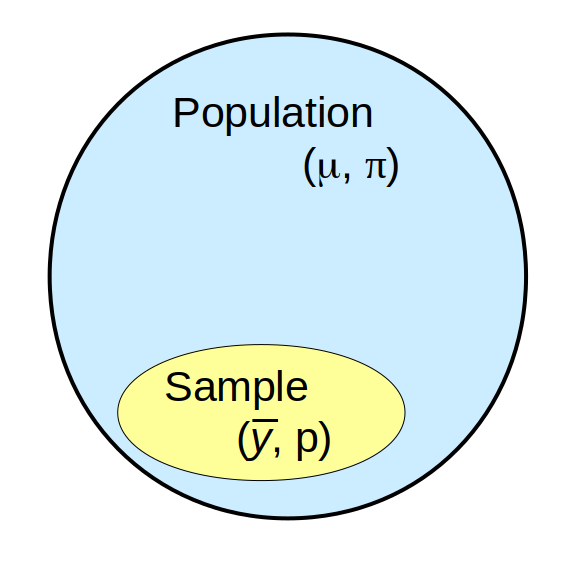
\includegraphics[scale=0.35]{MeansFig1.png}
	}
	
\end{frame}


\begin{frame}{The (statistical) parameters we will be concerned with: $\mu$}
	

\begin{itemize}
	\item $\mu$: The mean level of a quantitative characteristic, e.g. the depth of the earth's ocean or height of the land, or the height / BMI / blood pressure levels of a human population. \pause 
	\item One could also think of mathematical and physical constants as parameters, even though their values are effectively 'known.' Examples where there is agreement to many many decimal places include the mathematical constant pi, the speed of light (c), and the gravitational constant G. The speed of sound depends on the medium it is travelling through, and the temperature of the medium. The freezing and boiling points of substances such as water and milk depend on altitude and barometric pressure.  \pause 
	\item At a lower level, we might be interested in personal characters, such as the size of a person's vocabulary, or a person's mean (or minimum, or typical) reaction time. The  target could be a person's 'true score' on some test -- the  value one would get if one (could, but not realistically) be tested on each of the (very large) number of test items in the test bank, or observed/measured continously over the period of interest.  

\end{itemize}

\end{frame}



\begin{frame}{The (statistical) parameters we will be concerned with: $\pi$}
	
	
	\begin{itemize}
	
		\item $\pi$: Prevalence or risk (proportion): e.g.,  proportion of the earth's surface that is covered by water, or of a human population that has untreated hypertension, or lacks internet access, or will develop a new health condition over the next x years. \pause 
		\item At a lower level, we might be interested in personal proportions, such as what proportion of the calories a person consumes come from fat, or the proportion of the year 2020 the person spent on the internet, or indoors, or asleep, or sedentary.	
	\end{itemize}
	
\end{frame}





\begin{frame}{The (statistical) parameters we will be concerned with: $\lambda$}
	
	
	\begin{itemize}
			
		\item $\lambda$: The speed with which events occur: e.g., earthquakes per earth-day, or heart attacks or traffic fatalities per (population)-year. 
		\item At a lower level, we might be interested in personal intensities, such as the mean number of tweets/waking-hour  a person issued during the year 2020, or the mean number of times per 100 hours of use a person's laptop froze and needed to be re-booted.
		
	\end{itemize}
	
\end{frame}



\begin{frame}{The (statistical) parameters we will be concerned with}
	
	
	\begin{itemize}
		\item Each of these three parameters refers to a characteristic of the overall domain, such as entire surface of the earth, or the entire ocean, or population. There are no indicators for distinguishing among subdomains, so they refer to locations / persons not otherwise specified. We will drill down  later. \pause 
		
		\item Especially for epidemiologic research, and also more generally, one can think  of $\pi$ and $\lambda$ as  parameters of occurrence. [Although the word occurrence usually has a time element, it can also be timeless: how frequently a word occurs in a static text, or a mineral in a rock.] \pause 
		
		\item Prevalence is the proportion in a current state, and the 5-year risk is the expected proportion or probability of being in a new state 5 years from now. The  parameter $\lambda$ measures the speed with which the  elements in question move from the original to the other state.\pause 
		
		\item Even though the depths of the ocean, and blood pressures, are measured on a quantitative (rather than on all or none) scale, one can divide the scale into a finite number of bins/caterories, and speak of the prevalence (proportion) in each category. Conversely, one can use a set of descriptive parameters called quantiles, i.e, landmarks such that selected proportions, e.g., 0.05 or 5\%, 25\%, 50\%, 75\%, 95\% of the distribution are to the left of ('below') these quantiles.
	\end{itemize}
	
\end{frame}



\begin{frame}{Terminology}
\begin{itemize}
	\item Before we go on, we need to adopt sensible terminology for referring generically to the states, traits, conditions or behaviours  whose category-specific parameter values are being compared. \pause 
	
	\item We will use the term  \textbf{determinant}. It has several advantages over the many other terms used in different disciplines, such as exposure, agent, independent/explanatory variable, experimental condition, treatment, intervention, factor, risk factor, predictor. The main advantage is that it is broader, and closer to causally neutral in its connotaion. \pause 
	
	\item  \textit{Exposure} has environmental connotations, and technically refers to an opportity to injest or mentally take on board a substance or message.  
	\pause 
	\item The term \textit{independent variable} suggests the investigator has control over it in a laboratory setting. 
	\pause 
	\item The term \textit{explanatory} is  ambiguous as to the mechanism by which the parameter value in the index category got to be different from the value in the index category. Not all contrasts are experimentally formed. 

\end{itemize}
\end{frame}


\begin{frame}{Terminology}
	\begin{itemize}
		\item The term \textit{factor}, and thus the term \textit{risk factor}, are to be avoided because the word factor derives from the Latin \textit{facere}, (the action of) doing, making, creating. 
		\pause 		
		\item \textit{Predictor} makes one think of the future. 
		
		\pause 
		\item The term \textit{regressor} (or its shorthand, the 'X' ) won't be understood by lay people.
		
				\pause 
		\item While the word \textbf{determine} can suggest causality (e.g., demand determines the price), it also refers to 'fixing the form, position, or character of beforehand': two points determine a straight line; the area of a circle is determined by its radius.
		
				\pause 
		\item We now move on to the parameter relations we will be concerned with, beginning with the simplest type.
	\end{itemize}
\end{frame}



\begin{frame}{Parameter Contrasts}
	\begin{itemize}
		\item In applied research, we are seldom interested in a single constant. 
		
		
				\pause 
		
		\item Much more often we are interested in the contrast (difference) between the parameter values in different contexts/locations (Northern hemisphere vs Southern hemisphere), conditions/times (reaction times using the right versus left hand, or behaviour on weekdays versus weekends), or sub-domains or sub-populations (females vs males).
		
		\pause 
		
		\item In this section, we will limit our attention to 'contrasts': a compariosn of the parameter values between 2 contexts/locations/sub-populations. Thus the parameter function has just 2 possible 'input' values. 
	\end{itemize}
\end{frame}



\begin{frame}{'Reference' and 'Index' categories}
	\begin{itemize}
		\item In many research contexts, the choice of 'reference' category (starting point, the category against which the other category is compared) will be obvious: it is the \textbf{status quo} (standard care, prevailing condition or usual situation, dominant hand, better known category). 
		\pause 
		\item The 'index' category is \textbf{the category one is curious about} and wishes to learn more about, by contrasting its parameter value with the parameter value for the reference category.
		\pause 		
		\item In other contexts, it is less obvious which category should serve as the reference and the index categories, and the choice may be merely a matter of persepctive. If one is more famiar with the Northern hemisphere, it serves as a natural starting point 
		
				\pause 
		\item The choice of reference category in a longevity contrast between males and females, or in-hospital mortality rates or motor vehicle fatality rates during weekends versus weekdays, might depend on what mechanism one wishes to bring out. 
		
				\pause 
		\item Or one might chose as the reference category the one with the larger amount of experience, or maybe the one with the lower parameter value, so that the 'index minus reference' difference would be a positive quantity, or the 'index: reference ratio' exceeds 1.
	\end{itemize}
\end{frame}




\begin{frame}{'Reference' and 'Index' categories}
	\begin{itemize}
		\item The choice of reference category in a longevity contrast between males and females, or in-hospital mortality rates or motor vehicle fatality rates during weekends versus weekdays, might depend on what mechanism one wishes to bring out. 
		
		\item Or one might chose as the reference category the one with the larger amount of experience, or maybe the one with the lower parameter value, so that the 'index minus reference' difference would be a positive quantity, or the 'index: reference ratio' exceeds 1.
	\end{itemize}
\end{frame}



\begin{frame}{Parameter relations in numbers and words}
\begin{itemize}
\item To make this concrete, we will use hypothetical (and very round) numbers and pretend we 'know' the true parameter values -- in our example
of the mean depth of the ocean in the Northern hemisphere (reference category) and Southern hemisphere (index category) -- to be 3,600 metres (3.6Km) and 4,500 metres (4.5Km) respectively. Thus, the difference (South minus North) is 900 metres or 0.9Km.
\pause
\item If we wished to show the two parameter values graphically, we might do so using the format in panel (a), which shows the 2 hemisphere-specific parameter values -- but forces the reader to calculate the difference.

\item Panel (b) follows a more reader-friendy format, where the difference (the quantity of interest) is isolated:  the original 2 parameters are converted to 2 new, more relevant ones. 

\item Panel (c) encodes the relation displayed in panel (b) in a \textbf{single phrase} that applies to \textbf{both} categories: Onto the 'starting value' of 3.8Km, one \textbf{adds} $\Delta \mu$ = 0.9 Km \textbf{only if} the  resulting parameter pertains to the Southern hemisphere. The 0.9 Km is toggled off/on as one moves from North to South.   
\end{itemize}
\end{frame}




\begin{frame}[fragile,plain]

\begin{knitrout}\tiny
\definecolor{shadecolor}{rgb}{0.969, 0.969, 0.969}\color{fgcolor}

{\centering 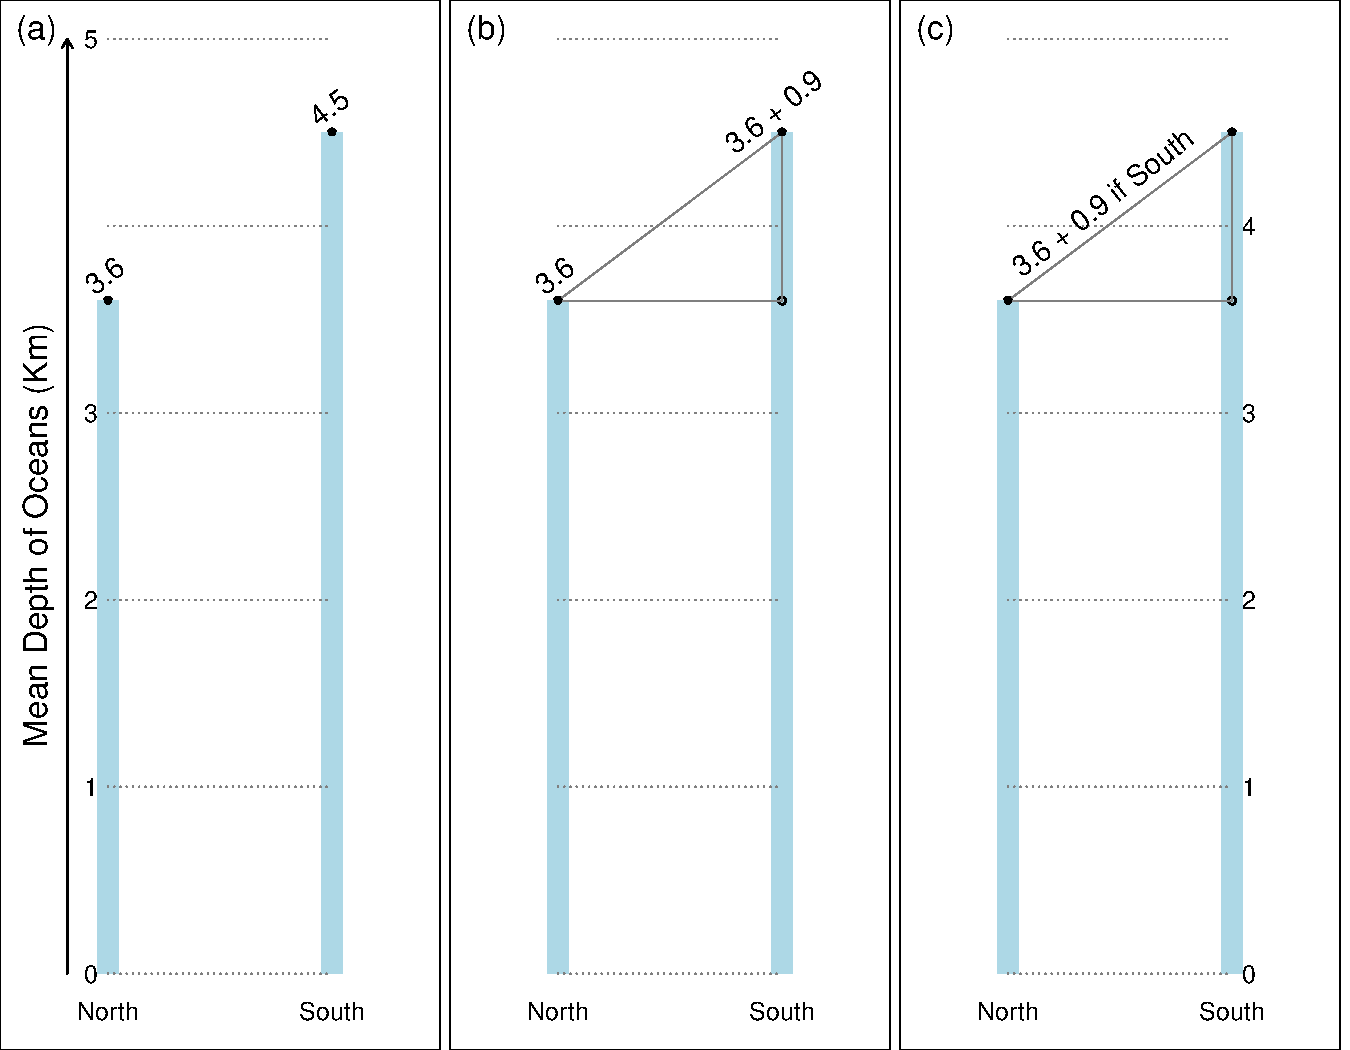
\includegraphics[width=\maxwidth]{figure/unnamed-chunk-1-1} 

}



\end{knitrout}
\end{frame}


\begin{frame}{Parameter relations in symbols, and with the help of an  index-category indicator}
\begin{itemize}
\item Panels (a) and (b) in the following figure repeat the information in panels (a) and (b) in the preceding Figure, but using Greek letters to symbolically represent the parameters. Just to keep the graphics uncluttered, the labels North and South are abbreviated to N and S and used as subscripts. Also, for brevity, the expression $\Delta \mu$ denotes $\mu_S - \mu_N$. 

\pause 

\item The relation encoded in a single phrase shown in the previous panel (c) has a compact form suitable for verbal communication. The representation can be adapted to be more suitable for computer calculations. (The benefit of doing this will become obvious as soon as you try to learn the parameter values by fiiting these models to actual data.) Depending on whether the hemisphere in question is the northern or southern hemisphere, the expression/statement 'the specified hemisphere is the SOUTHERN hemisphere' evaluates to a (logical) FALSE or TRUE. In the binary coding used in computers, it evaluates to 0 or 1, and we call such a 0/1 variable an 'indicator' variable.



\end{itemize}	
	
\end{frame}




\begin{frame}{Parameter relations in symbols, and with the help of an  index-category indicator}
	\begin{itemize}
		\item In panel (c) in the following figure, just to keep the graphics uncluttered, the name of the indicator variable SOUTHERN is abbreviated to S, and $\mu_S$ is shorthand for the $\mu$ cooresponding to whichever value (0 or 1) of $S$ is specified (we could also write it as $\mu | S$, or $\mu$ 'given' $S$.) Thus, the symbol $\mu_0$ refers to the $\mu$ when $S=0$, or in longerhand, to $\mu \ | \ S = 0$. 
		
	\end{itemize}	
	
\end{frame}



\begin{frame}[fragile,plain]
\begin{knitrout}\tiny
\definecolor{shadecolor}{rgb}{0.969, 0.969, 0.969}\color{fgcolor}

{\centering 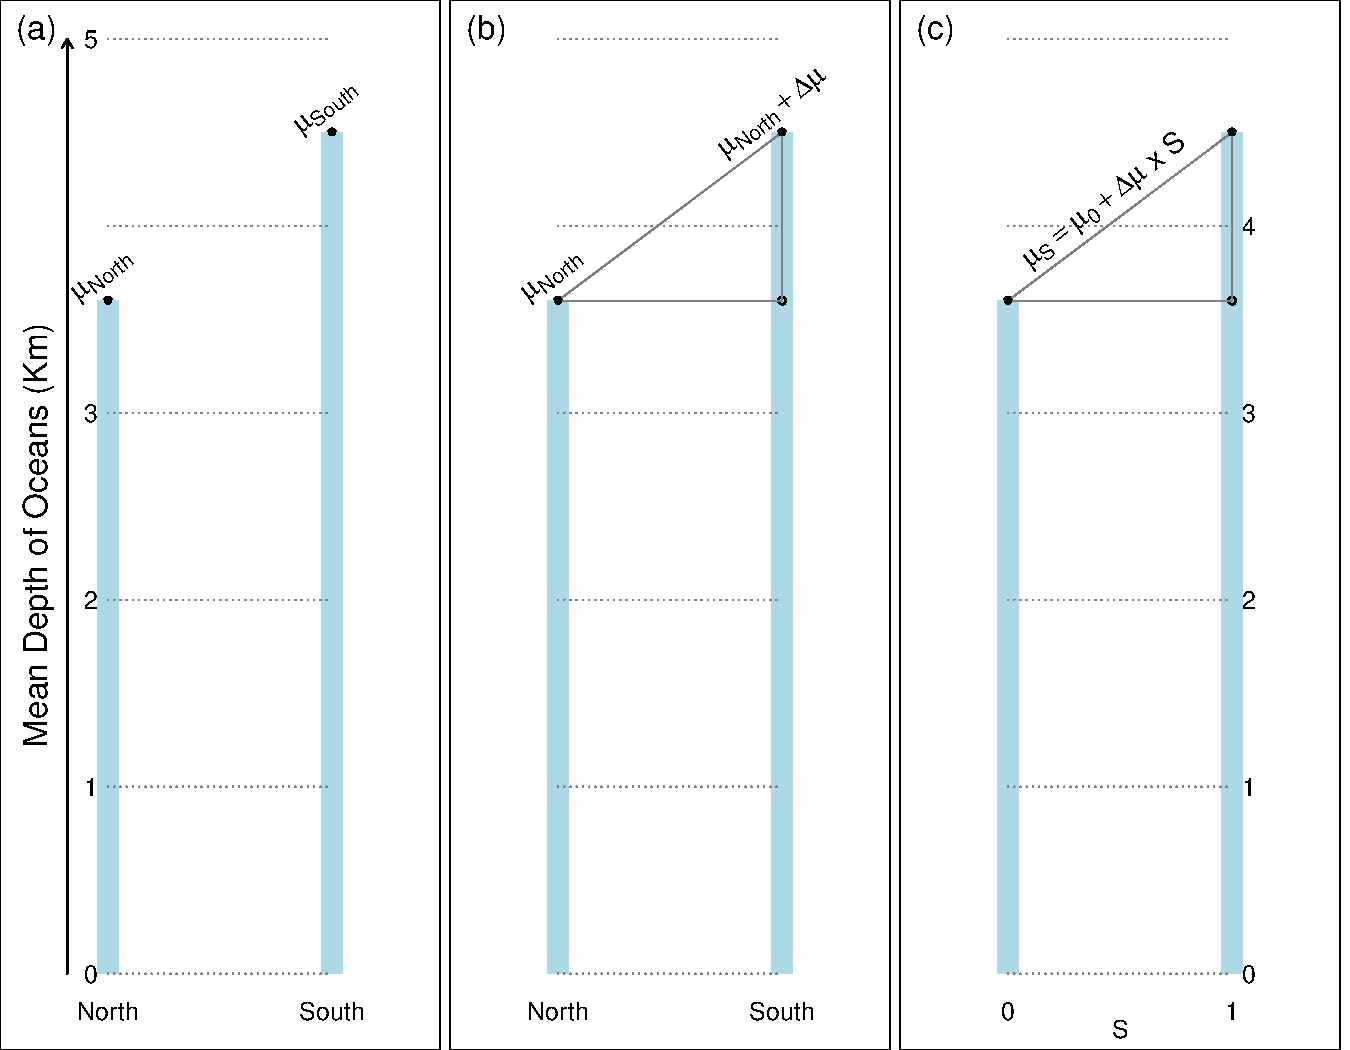
\includegraphics[width=\maxwidth]{figure/unnamed-chunk-2-1} 

}



\end{knitrout}
\end{frame}




\begin{frame}{Relative differences (ratios) - in numbers}
\begin{itemize}
	\item A ratio can be more helpful than a difference, especially if you are don't have a sense of how large the parameter value is even in the reference category. As an example, on average, how many more red blood cells do men have than women? or how much faster  are gamers' reaction times compared with nongamers?
\pause 
\item Recall our hypothetical mean ocean depths, 3.6 Km  in the 
oceans in the Northern hemisphere (reference category) and 4.5Km in the oceans of the Southern hemisphere (index category). Thus, the S:N (South divided by North) ratio is 4.5/3.6 or 1.25.
\pause 
\item Panel (a) leaves it to the reader to calculate the ratio of the parameter values. In panel (b)  the ratio (the quantity of interest) is isolated:  again, the original 2 parameters are converted to 2 new, more relevant ones. 
\pause 
\item Again, panel (c) shows a single master-equation that applies to both hemispheres by togging off/on the ratio of 4.5/3.6.
\end{itemize}
\end{frame}


\begin{frame}[fragile,plain]
\begin{knitrout}\tiny
\definecolor{shadecolor}{rgb}{0.969, 0.969, 0.969}\color{fgcolor}

{\centering 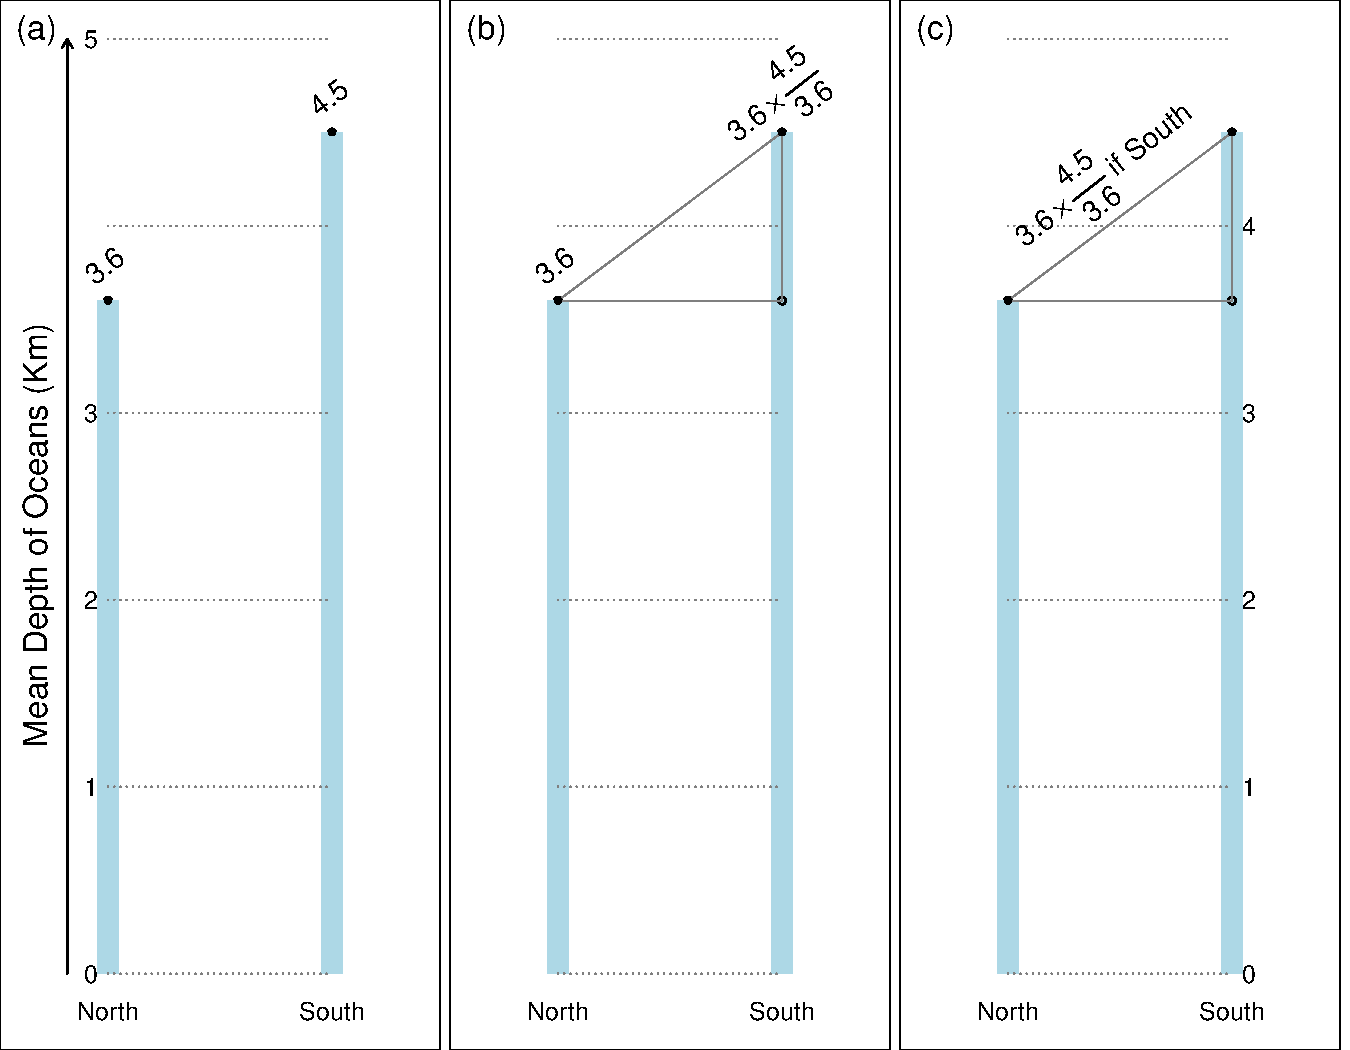
\includegraphics[width=\maxwidth]{figure/unnamed-chunk-3-1} 

}



\end{knitrout}
\end{frame}





\begin{frame}{Relative differences (ratios) - expressed in symbols}
	\begin{itemize}
		\item To rewrite these numbers in a symbolic equation suitable for a computer, we  again convert the logical 'if South' to a numerical Southern-hemisphere-indicator, using the binary variate $S$ (short for Southern) that takes the value 0 if the Northern hemisphere, and  1 if the Southern hemisphere.
		\pause 
	\item 	But go back to  some long-forgotten mathematics from high school to be able to tell the computer to toggle the ratio off and on. Recall \textbf{powers} of numbers, where, for example, 
		'$y$ to the power 2', or $y^2$ is the square of $y$. The two powers we exploit are 0 and 1.
		'$y$ to the power 1', or $y^1$ is just $y$ and '$y$ to the power 0', or $y^0$ is 1.
		\pause 		
\item 		We take advantage of these to write
		$$\mu_S = \mu \ | \ S  \ = \mu_0 \ \times \  \Big\{ \frac{\mu_{South}}{\mu_{North}}\Big\}^S = \mu_0 \ \times Ratio \ ^ S.$$ 
		
	\item 	You can check that it works for each hemisphere by setting $S=0$ and $S=1$ in turn. Thus, $$\log(y^S) = S \times \log(y)$$  
		
	\end{itemize}
\end{frame}


\begin{frame}[fragile,plain]
\begin{knitrout}\tiny
\definecolor{shadecolor}{rgb}{0.969, 0.969, 0.969}\color{fgcolor}

{\centering 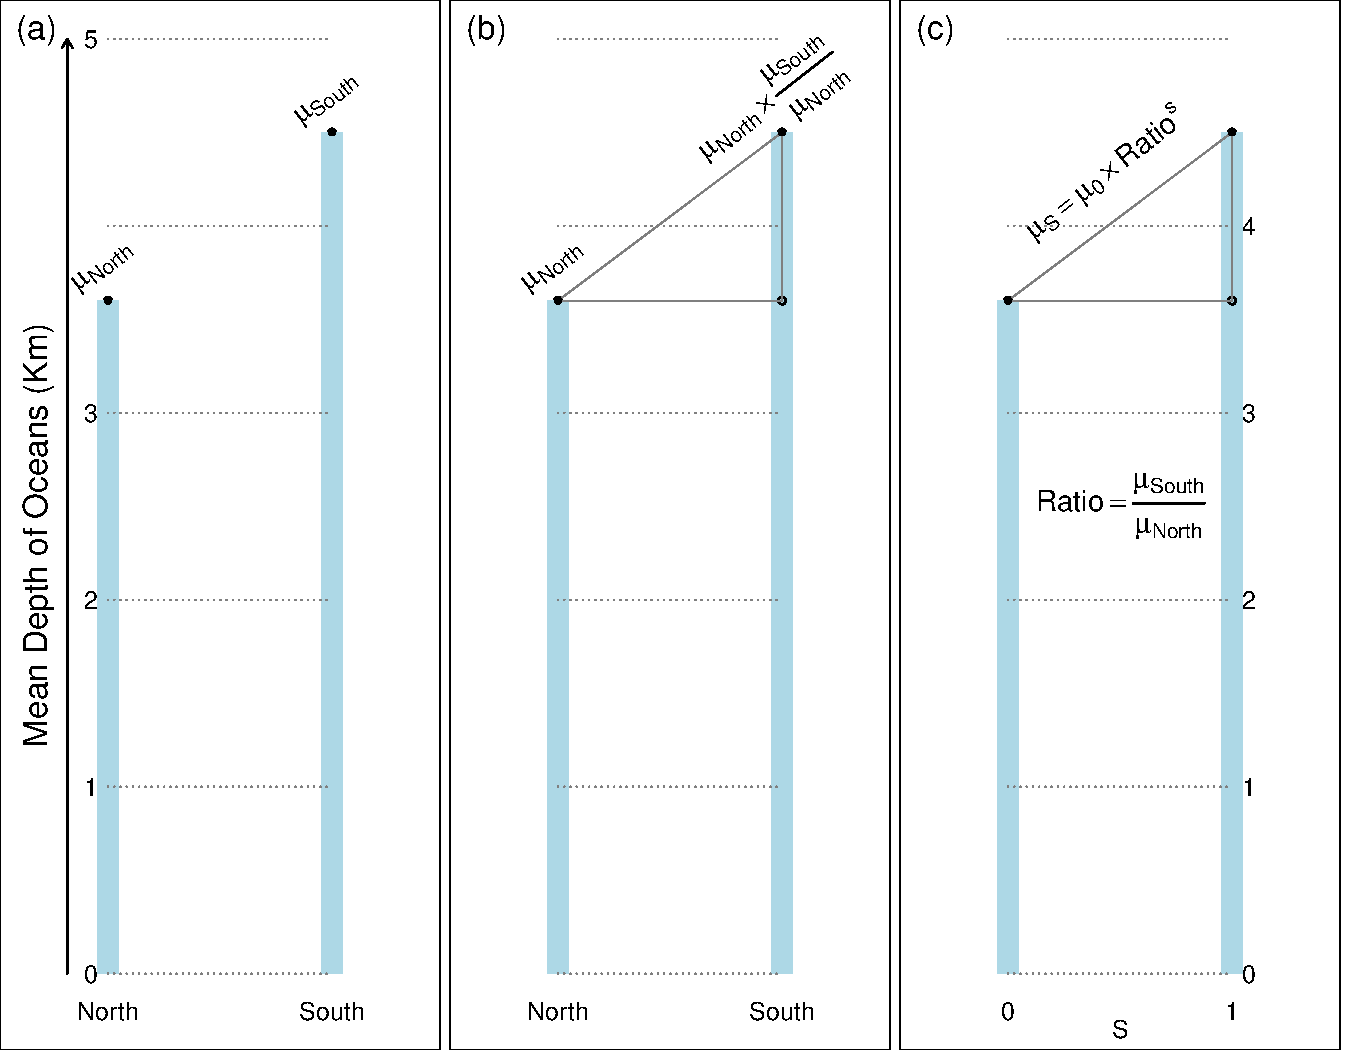
\includegraphics[width=\maxwidth]{figure/unnamed-chunk-4-1} 

}



\end{knitrout}
\end{frame}



\begin{frame}
\begin{itemize}
	\item Although this is a compact and direct way to express the
	parameter relation, it is not well suited for fitting these equations to data. 
	
\item 	However, in those same  high school mathematics courses, you also learned about \textbf{logarithms}. For example, that 
	$$\log(A \times B) = \log(A) + \log(B); \ \  \log(y^x) = x \times \log(y).$$
	\pause 
	\item Thus, we can rewrite the equation in panel (c) as
	
	$$\log(\mu_S) = \log(\mu \ | \ S)  \ = \underbrace{\log(\mu_0)} \ +  \underbrace{\log(Ratio)} \times \ S.$$
	
	\item This has the same 'linear in the two parameters' form as the one for the parameter difference: the parameters are
	$\underbrace{\log(\mu_0)}$ and $\underbrace{\log(Ratio)}$ and they are made into the following 'linear compound' or 'linear predictor' (see Remarks below) :
	$$\log(\mu_S) = \log(\mu \ | \ S)  \ = \underbrace{\log(\mu_0)} \times \ 1 \ + \underbrace{\log(Ratio)} \times \ S.$$
	\pause 
\item 	The course is concerned with using 'regression' software to  'fit'/'estimate' these 2 parameters from $n$ depth measurements indexed by $S$.
	
\end{itemize}
\end{frame}


\begin{frame}{Parameter Functions}
\begin{itemize}
	\item A very simple example of a function that describes how  parameter values vary over quantitative levels of a determinant is the straight line shown in the upper right panel of the next figure. Here the determinant has the generic name X, and the equation is of the $A + B \times X$ or $B_0 + B_1 \times X$ or $\beta_0 + \beta_1 \times X$ straight line form. 
	
	\item Miettinen used the convention that the upper case letters $A$ and $B$ are used to denote the (true but unknown) coefficient values, whereas the lower case leters $a$ and $b$ are used to denote their empirical counterparts, sometimes called estimated coefficients or fitted coefficients.  This sensible and simple convention also avoids the need, if one uses Greek letters for the theoretical coefficient values, to put 'hats' on them when we refer to their empirical counterparts, or 'estimate/fit' them. Fortunately, journals don't usually allow investigators to use 'beta-hats'; but this means that the investigators have to be more careful with their words and terms.
	

\end{itemize}
\end{frame}


\begin{frame}{Parameter Functions}
	\begin{itemize}
		
		\item As we go left to right in the following grid, the models become more complex. The simplest  is the one of the left, in column 1, the one  JH refers to as 'the mother of all regression models.'  It refers to a \textit{single} or \textit{overall} situation/population/domain, so $X \equiv 1$, it takes on the value 1 in/for every instance/member. 
		
		
		\item So the parameter equation is $\mu_X = \mu \ | \ X \ = \mu \times 1.$ In column 2, there are 2 subdomains, indexed by the 2 values of  the determinant (here generically called 'X'), namely $X = 0$ and $X = 1$. In the 3rd column, the number of of parameters is left unspecified, since the numbers of coefficients to specify a line/curve might vary from as few as 1 (if we were describing how the volume of a cube dependeds or, was is function of, its radius) to 2 (for a straight line that did not go through the origin, or for a symmetric S curve) to \textit{more than 2} (e.g., for a non-symmetric S curve, or a quadratic shape).
	\end{itemize}
\end{frame}


\begin{frame}[fragile,plain]
\begin{knitrout}\tiny
\definecolor{shadecolor}{rgb}{0.969, 0.969, 0.969}\color{fgcolor}

{\centering 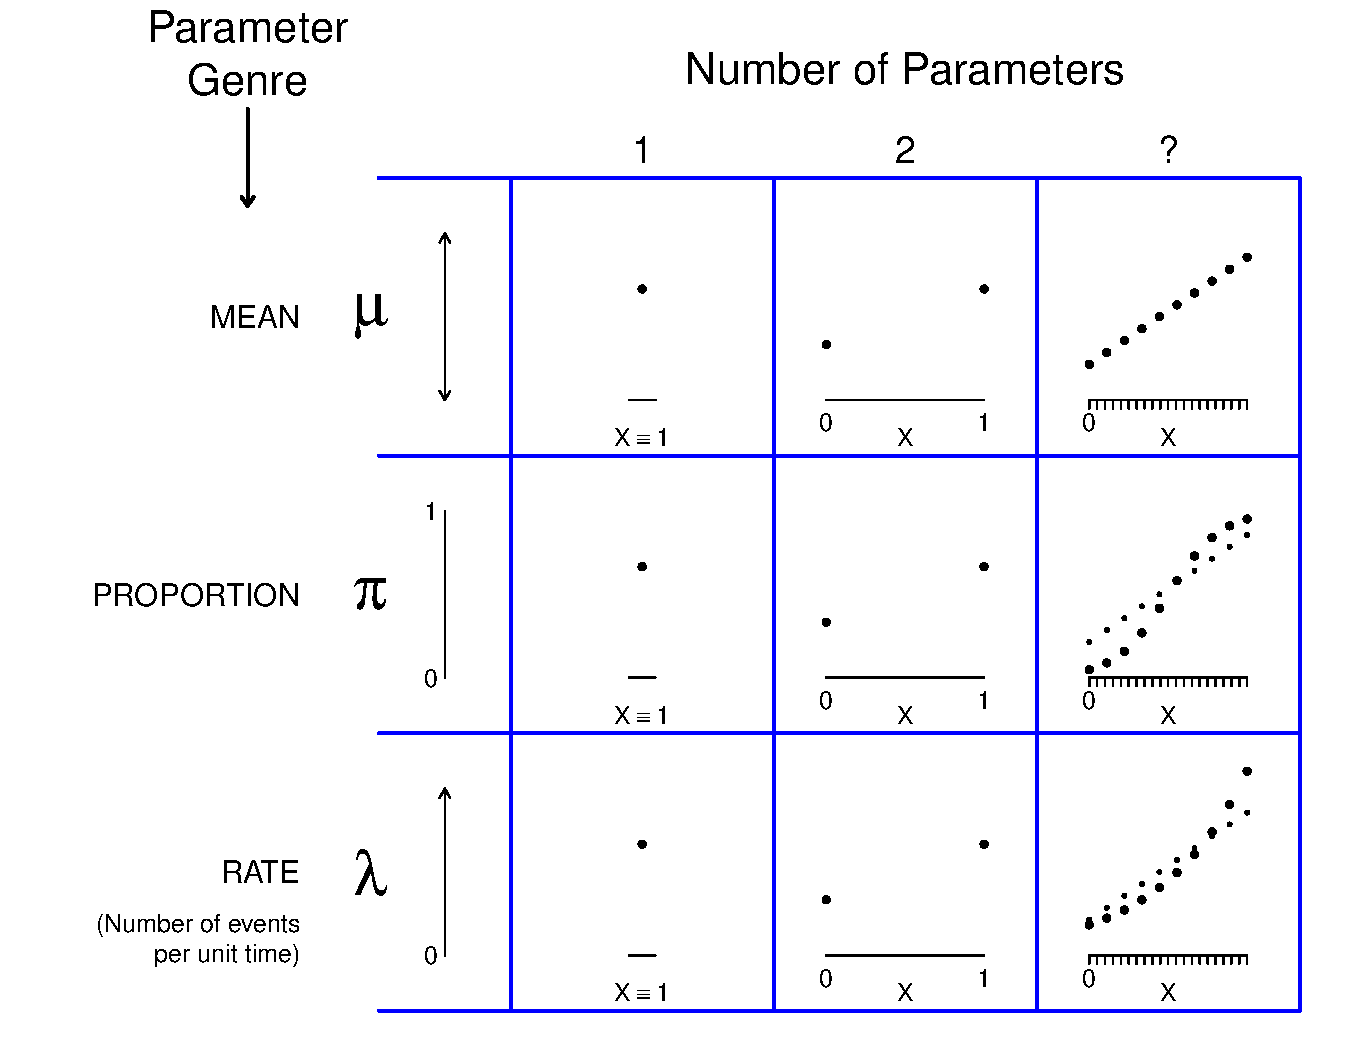
\includegraphics[width=\maxwidth]{figure/unnamed-chunk-5-1} 

}



\end{knitrout}
\end{frame}


\end{document}


